\chapter{Support for a new board}

\section{Context}
One of our clients wants to release a new version of its product in a midterm future. They sent an evaluation board so we could work on adding support for this board in both Linux and U-Boot.

An evaluation board is a board which is offered by some vendors to other vendors to build a beta version of the new product they want to release. The main advantage is the possibility to test the software stack before building the hardware. This means they can test the software stack before building the multiple beta iterations of their product's hardware and test the hardware they thought would meet their needs actually does. After the hardware has been validated, they can change its form-factor and adjust the software to reflect those changes. In short, the evalutation board is a must-have in the creation process of a product: it saves both money and time by not having to actually build your product to be able to test it.

The new version of the product will share most of its components with the Allwinner Parrot EVB R16, the evaluation board we have to add support for. This board is shipped with one of the newest SoCs of Allwinner, the R16 which is assumed to be very close to an Allwinner A33 SoC. We assume this closeness with the A33 because there is no publicly available documentation yet for this SoC but the few information we have let us guess it is sharing a lot of similarities with the A33.

Yet, there is no support for the Allwinner Parrot EVB R16 in either the Linux kernel or U-Boot, but fortunately, the A33 is supported in both projects. Since they are assumed to be pretty much the same SoC, we can start from the files needed by the A33 and tweak them bit by bit to make all the components work.

The goals of this project are first to be able to interact with the U-Boot bootloader in order to then boot a Linux kernel.

\section{Project}

\begin{figure}[H]
  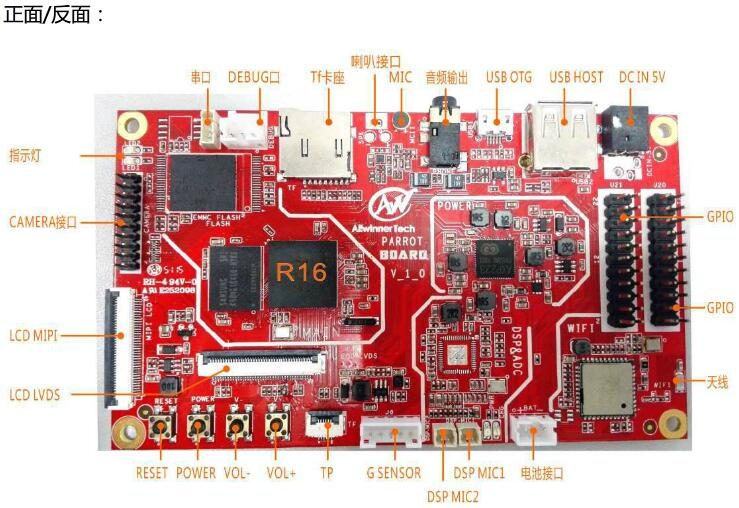
\includegraphics[width=\textwidth]{parrot_r16.jpg}
  \caption{The Allwinner Parrot EVB R16 and all its components}
\end{figure}

The Parrot Board is an evaluation board with an Allwinner R16 (assumed to be close to an Allwinner A33), 4GB of eMMC\footnote{\url{https://en.wikipedia.org/wiki/MultiMediaCard\#eMMC}}, 512MB of RAM, USB host and OTG\footnote{\url{https://en.wikipedia.org/wiki/USB\_On-The-Go}}, a WiFi/Bluetooth combo chip, a micro SD card reader, 2 controllable buttons, two controllable LEDs, an LVDS port (mainly for use with an LCD) with separated backlight and capacitive touch panel ports, an audio/microphone jack, a camera CSI port, 2 sets of 22 GPIOs and an accelerometer.

\subsection{Add support in the bootloader source code}
To support a new board, the first and most important step is to have a working bootloader from which we will later be able to boot the Linux kernel. There are multiple open source bootloaders\footnote{\url{https://en.wikipedia.org/wiki/Comparison\_of\_boot\_loaders}} available but only a few are widely used. At Free Electrons, we work substantially with U-Boot\footnote{\url{http://www.denx.de/wiki/U-Boot/}} and in few occasions with Barebox\footnote{\url{http://www.barebox.org/}}. U-Boot is today the most widely used bootloader in embedded systems.

All boards host a small ROM code which is embedded in the processor and whose only purpose is to load in SRAM\footnote{Static Random Access Memory} a file from a fixed location (be it on the SD card or the internal storage). Because the SRAM is often really limited on a system, being more expensive than DRAM\footnote{Dynamic Random Access Memory}, this ROM code loads a first-stage bootloader which has a few functionalities, the most important being the initialization of the DRAM. This first-stage bootloader (or SPL\footnote{Secondary Program Loader}) will then initialize the DRAM and loads the full, or second-stage, bootloader in it. Yet, some boards embed enough SRAM to load a full bootloader so the SPL is not needed.

In Allwinner SoCs (named sunxi), the SRAM is too small to load a full bootloader, so we need a SPL. U-Boot can build an SPL and a full bootloader from the same compilation command so we do not have to worry on building it. The next step is to find on which pins of the board the serial communication is working so we can communicate with the bootloader of the board (if there is one). Once that's done, we have to figure a way to place the bootloader we'll compile in one of the locations the ROM code will try to load the bootloader from. On Allwinner SoCs, we can either write on the internal storage by entering the FEL mode\footnote{\url{http://linux-sunxi.org/FEL}} or create a bootable SD card\footnote{\url{http://linux-sunxi.org/Bootable\_SD\_card}}. Entering the FEL mode is a board specific manipulation and, unfortunately, I did not have enough documentation on the board to enter in such mode. Therefore, everytime I compiled a new bootloader, I had to recreate a bootable SD card with the newest SPL and full versions of U-Boot.

Here is the process of creating a bootable SD card for Allwinner SoCs:
\begin{enumerate}
  \item compile U-Boot,

\begin{minted}[linenos=true,bgcolor=grey,numberblanklines=true,breaklines=true]{console}
$ make CROSS_COMPILE=arm-linux-gnueabihf- my_config
$ make CROSS_COMPILE=arm-linux-gnueabihf- -j$(nproc)
\end{minted}

  \item identify the SD card device name,

\begin{minted}[linenos=true,bgcolor=grey,numberblanklines=true,breaklines=true]{console}
$ dmesg
[59358.008977] mmc0: new high speed SDHC card at address b368
[59358.019617] mmcblk0: mmc0:b368 NCard 3.72 GiB
\end{minted}

  \item erase the part of the SD card with the SPL bootloader,

\begin{minted}[linenos=true,bgcolor=grey,numberblanklines=true,breaklines=true]{console}
# dd if=/dev/zero of=/dev/mmcblk0 bs=1M count=1
\end{minted}

  \item write the SPL version of U-Boot to the SD card,

\begin{minted}[linenos=true,bgcolor=grey,numberblanklines=true,breaklines=true]{console}
# dd if=u-boot-sunxi-with-spl.bin of=/dev/mmcblk0 bs=1024 seek=8
\end{minted}

  \item partition the SD card,

\begin{minted}[linenos=true,bgcolor=grey,numberblanklines=true,breaklines=true]{console}
# blockdev --rereadpt ${card}
cat <<EOT | sfdisk ${card}
1M,16M,c
,,L
EOT
\end{minted}

We'll then have two partitions: mmcblk0p1 for data accessible by U-Boot SPL and full bootloader and mmcblk0p2 for external storage.

  \item format partitions,

\begin{minted}[linenos=true,bgcolor=grey,numberblanklines=true,breaklines=true]{console}
# mkfs.vfat /dev/mmcblk0p1
# mkfs.ext4 /dev/mmcblk0p2
\end{minted}

This will format the first partition in FAT and the second in EXT4.

  \item copy the full bootloader to the SD card,

\begin{minted}[linenos=true,bgcolor=grey,numberblanklines=true,breaklines=true]{console}
# mount /dev/mmcblk0p1 /mnt
# cp u-boot.bin /mnt
# umount /mnt
\end{minted}
\end{enumerate}

The U-Boot bootloader needs to be compiled with rightly configured settings so it is compiled for the correct architecture, and can find how to configure the RAM, the USB ports, the internal storage and so on.

The first settings to get right are the architecture (ARM and Allwinner SoC) and the DRAM initialization. These settings' value can be found in vendor documents. Once we have a bootloader which boots without errors, we can add bit by bit new settings to enable more components. Between each compilation, it is important to test the bootloader and all its components on the board to see if we are not introducing regressions.

The core components of the bootloader are the one which can be used to load files from external storage, internal storage and other devices. Without these, it is impossible to make a kernel boot since we cannot get the file in the bootloader. U-Boot can get files from NAND, eMMC, SD card, USB from USB sticks or fastboot, the network via TFTP and serial. On the Allwinner Parrot EVB R16, we have 4GB of eMMC, an USB host port, a micro USB OTG port and a micro SD card reader which can help to retrieve files. We could use the USB OTG port to simulate a network interface in the bootloader and get files over the network via TFTP.

Once we get all those important components, we can send the new files and modifications to the U-Boot community so they can review it, comment it, maybe ask for some modifications and validate it so it can be added to the source code.

\subsection{Add support in Linux kernel source code}

The client wanted an initial support in the kernel. The aim is to make the kernel detect hardware components and map them to existing drivers. If a component does not have yet an existing or working driver, there is no need to develop one at the moment. However, all important components such as USB ports, WiFi and Bluetooth chip, the internal storage and the micro SD card reader have to work or the board is almost unusable for end users.

As presented before, the R16 is assumed to be close to the A33 and most components of the Parrot EVB R16 are also in the Sinlinx SinA33 (which embeds an A33). The easiest and most straight-forward process is to start from the files needed for the Sinlinx SinA33, strip all its components leaving only the ones required to boot and add component by component until everything is included.

There would have been more files required if the SoC was not actually close to a known one, but fortunately the only needed file to make the kernel boot is a Device Tree file. The Device Tree is, as its name suggests, a tree of devices and is a representation of hardware devices and buses which are present in a board and are not discoverable at runtime. This file is compiled beside the Linux kernel with the Device Tree Compiler and a change in its code does neither affect the kernel nor requires a rebuild of the kernel. A Device Tree Blob is created once the Device Tree has been compiled and has to be used in conjunction with a compiled kernel or the kernel will not be able to boot. A Device Tree is specific to one board but can inherit components' definition from Device Trees includes.

The Device Tree is a file organized like a tree, with a root node, bus nodes and devices nodes. The root node typically contains a \textit{cpus} node describing each CPU in the system, a \textit{memory} node defining the location and size of the RAM, an \textit{aliases} node specifying shortcuts to some nodes, and nodes describing SoC buses such as USB, i\textsuperscript{2}c or SPI and on-board devices such as LEDs, eMMC, SD card reader, Ethernet port or power regulators.

Each node (even the root node) has a \textit{compatible} property which is used by drivers to know if they can manage and interact with the hardware device represented by this node. When a driver is mapped to one or more nodes, it can access all settings defined in these nodes. The goal is to give as many relevant information as possible in the Device Tree nodes so the drivers have enough data to know how to handle the device. These information can be links to other nodes (power regulators or pin muxing for example), to hardware interrupts or address of registers.

The first node to add is the node in charge of the UART device which is used to communicate with the board via serial. If this node is wrongly set, we would not be able to interact with the kernel which is absolutely useless. Once this device is correctly set, we can add more components such as the USB port, the SD card reader, WiFi and Bluetooth chip, power regulators and the micro USB OTG port.

Two of the things to keep in mind when writing a Device Tree file are pin muxing and power regulators. In a SoC, there is only a limited number of pins in order to make the SoC as small as wished by the vendor but there are a lot of hardware components on the board. These two statements seem to be completely opposite but pin muxing exists to make them possible at the same time. Pin muxing is a hardware workaround which allows multiple hardware components to be wired on the same pin of the SoC. The SoC decides which hardware component has the right to communicate with it through this pin and blocks all other components linked to the same pin. This obviously needs some thinking when designing the board because two (or more) components on the same pin cannot work at the same time. It would be a shame to have both the USB ports and the WiFi chip on the same pins for example.\\
On a board, components are not all powered with the same voltage and sometimes accept voltages in a certain range or only a fixed voltage. If we mess up the power regulators in the Device Tree, we can burn components. Having a voltages range in some power regulators is useful when trying to reduce consumption of a component or make it temporarily more powerful.

\section{Conclusion}

Adding support for the Allwinner Parrot EVB R16 in both U-Boot and Linux kernel were my first interactions with the Linux and U-Boot communities. These interactions made me realise how important it is to ask other persons to comment, criticize, discuss and validate my code.

For this project, the different struggles were the lack of proper documentation (only electrical schematics and a FEX file\footnote{\url{http://linux-sunxi.org/Fex\_Guide}} which were sometimes contradicting each other and the need to rewrite the SD card each time a change was made to U-Boot. The rewriting of the SD card was painfully slow when adding support for the board in U-Boot.

To sum up, the initial support for this board has been added to U-Boot \footnote{\url{http://lists.denx.de/pipermail/u-boot/2016-June/258992.html}} and Linux kernel\footnote{\url{https://patchwork.kernel.org/patch/9197239/}}. However, the support for the accelerometer was not added since the documentation does not mention any brand or model name and I could not find it by trying to guess it.
